\documentclass[12pt,a4 paper]{book}
\usepackage[utf8]{inputenc}
\usepackage[english,russian]{babel}
\usepackage{misccorr}
\usepackage{graphicx}
\usepackage{amsmath}
\usepackage{mathtext}
\textwidth=17.2cm
\textheight=25cm
\oddsidemargin=--6mm
\evensidemargin=--6mm
\topmargin=--1mm

\usepackage{mathtools}
\usepackage{setspace}
\usepackage{amsfonts}
\usepackage[T2A]{fontenc}

\usepackage{graphicx}
\graphicspath{{pictures/}}
\DeclareGraphicsExtensions{.pdf,.png,.jpg}

\begin{document}
\begin{titlepage}
\begin{center}
\normalsize
МИНИСТЕРСТВО ОБРАЗОВАНИЯ И НАУКИ \\РОССИЙСКОЙ ФЕДЕРАЦИИ
\vspace{0.25cm}

МОСКОВСКИЙ ГОСУДАРСТВЕННЫЙ УНИВЕРСИТЕТ\\ им М.В.Ломоносова
\vspace{0.25cm}

Механико-математический факультет

Кафедра теории вероятностей
\vfill

\vfill

\textsc{\textbf{Курсовая работа}}\\[3mm]

{ “Принцип безарбитражности на примере опционов и свопов, 2” \\ "The principle of non-arbitrage on the example of options and swaps, 2" \\ }
\bigskip

\end{center}
\vfill

\newlength{\ML}
\settowidth{\ML}{«\underline{\hspace{0.7cm}}» \underline{\hspace{2cm}}}
\hfill\begin{minipage}{0.4\textwidth}
\textbf{Выполнил:}\\ студент 3 курса 331 группы\\ Ковальчук А.А.

\end{minipage}%
\bigskip

\hfill\begin{minipage}{0.4\textwidth}
\textbf{Научный руководитель:}\\ доц. кафедры теории веротностей\\ Жуленёв С.В.
\end{minipage}%
\vfill

\begin{center}
\vfill

\vfill
Москва, 2020 г.
\end{center}
\end{titlepage}

\thispagestyle{empty}

\smallskip
\begin{center}
{\bf\Large Содержание}
\end{center}
\begin{enumerate}
\item[1] \textbf{Введение} 

\item[2] \textbf{Принцип безарбитражности на примере опционов}
\begin{enumerate}
\item[2.1.] Постановка задачи
\item[2.2.] Решение
\end{enumerate}
\item[3] \textbf{Принцип безарбитражности на примере свопов}
\begin{enumerate}
\item[3.1.] Постановка задачи
\item[3.2.] Решение
\end{enumerate}
\item[4] \textbf{Список используемой литературы}
\end{enumerate}

\newpage
\section*{1. Введение}
\smallskip
\\В классической финансовой математике принцип безарбитражности является основополагающим. Также он играет важную роль в стохастической финансовой математике. Суть принципа можно изложить кратко: это принцип, при котором на рынке отсутствуют арбитражные возможности, то есть возможности безрискового перевода средств с одного рынка на другой с целью использования разницы в процентных ставках, обменных курсах или товарных ценах. Однако суть и значимость самого принципа можно понять только на конкретных примерах. В данной работе принцип безарбитражности будет разбираться на примере опционов и свопов, путем решения конкретных задач.

\newpage
\section*{2. Принцип безарбитражности на примере опционов}
\smallskip
\begin{enumerate}
\item[2.1.] \textbf{Постановка задачи}
\\
\\Введём следующие обозначения:
\smallskip
\begin{itemize}
    \item $S_t$ - стоимость 1 акции, т.е. базового актива на момент $t$, $S_0 = S$
    \item$P_t$ - стоимость опциона “пут” на момент времени $t$, $P_0=P$
    \item$C_t$ - премия продавца $-$ стоимость опциона “колл” на момент времени $t$, $C_0=C$
    \item$T$ - момент предъявления опциона к исполнению,
    $(0,Т)$ - срок жизни опциона
    \item $К$ - цена исполнения опциона
    \item$\tau=T-t$, где $t$ произвольный момент времени срока жизни опциона
    \item$\nu$ - ежегодная безрисковая ставка непрерывного начисления
    \item$f_T$ - платежное обязательство или выгода в момент времени t, которую владелец может получить в этот момент, $f_T=(S_t-K)^{+}$
\end{itemize}
\smalskip
\\ Необходимо привести другое доказательство леммы 2.7 из [1]. Правое неравенство в (2.5) необходимо вывести из принципа безарбитражности. А именно, мы будем доказывать правую часть неравенства:
\begin{center}
    $S_t - K <= C^{A}_t-P^{A}_t<=S_t - Ke^{-\nu\tau}$
\end{center}

\item[2.2.] \textbf{Решение}
\smallskip
\\\textbf{1.} Левая часть неравенства доказана в [1]. Докажем правую часть неравенства через принцип безарбитражности. То есть покажем, что $C^{A}_t-P^{A}_t<=S_t - Ke^{-\nu\tau}$.\\
    \textbf{2.} Предположим, что данное неравенство не выполняется, то есть $L \equiv C^{A}_t - P^{A}_t -S_t+Ke^{-\nu\tau}>0$. Тогда совершаем следующие действия для получения арбитражной прибыли:
    \begin{itemize}
        \item Покупаем опцион “пут” (его стоимость равна $P^{A}_t$)
        \item Покупаем акцию (её стоимость равна $S_t$)
        \item Продаем опцион “колл” (его стоимость равна $C^{A}_t$)
        \item Берем в долг сумму $Ke^{-\nu\tau}$
    \end{itemize}
    Итого имеем: $C^{A}_t+Ke^{-\nu\tau} - P^{A}_t -S_t \equiv L > 0$ (по предположению). Далее для получения арбитражной прибыли кладём выручку на счет в банк.\\
    \textbf{3.} Если владелец опциона “колл” исполнит его в некоторый момент $\theta, t<\theta<=T$, то так как $S_{\theta}>K$, то мы отдаем ему акцию за сумму $K$ и кладём ее на счёт. В результате, возвращая долг $K$ в момент времени $T$, остаемся с суммой на счету $K(e^{\nu(T-\theta)}-1)+Le^{\nu\tau}$.\\
    \textbf{4.} Если же опцион “колл” не исполняется, т.е. $S_T < K$, то мы можем продать акцию за $K$, исполняя тем самым опцион “пут”, и,возвращая долг в момент T, остаёмся с суммой $Le^{\nu\tau}$.\\
\end{enumerate}

\newpage
\section*{3. Принцип безарбитражности на примере свопов}
\smallskip
\begin{enumerate}
\item[2.1.] \textbf{Постановка задачи}
\\Компания $X$ желает занять американские доллары по фиксированной ставке. Компания $Y$ желает взять в долг японские иены по фиксированной ставке. Суммы, необходимые компаниям, с учетом текущего валютного курса приблизительно одинаковы. Процентные ставки по кредитам с учетом налогов приведены в следующей таблице.
		\begin{center}
		\begin{tabular}{|c||cc|}
			\hline
			& Иенна & Доллары\\
			\hline
			\hline
			Компания $X$ & 5.0$\%$  & 9.6$\%$  \\
			Компания $Y$ & 6.5$\%$  & 10$\%$  \\
			\hline
		\end{tabular}
		\end{center}
		Необходимо разработать своп, приносящий банку, действующему, как посредник, 50 базисных пунктов в год (1 базисный пункт = 0.01$\%$) и одинаково выгодный для обоих компаний. Необходимо также учесть риски, связанные с колебаниями валютного курса.
\item[2.2.] \textbf{Решение}
\smallskip
\\\textbf{1.} Для начала необходимо определить, имеются ли предпосылки для заключения взаимовыгодного свопа между компаниями $X$ и $Y$. По таблице определяем, что компания $X$ имеет сравнительное приемущество на рынке иен, но собирается приобретать доллары. Аналогично компания $Y$ имеет сравнительное приемущество на долларовом рынке, но собирается приобретать иены. Таким образом, появляются предпосылки для свопа.\\
		\textbf{2.} По таблице определяем, что ежегодная разница в курсах для иены равна 1.5$\%$ и 0.4$\%$ для доллара. Таким образом, общий выигрыш от заключения свопа равен 1.5$\%$ - 0.4$\%$ = 1.1$\%$ ежегодно.\\
		\textbf{3.} Банк требует 50 базисных пунктов или 0.5$\%$ ежегодно. Следовательно, на $X$ и $Y$ остается по (1.1$\%$-0.5$\%$):2 = 0.3$\%$ на каждую. Следовательно, имеем, что своп должен давать возможность для компании $X$ взять доллары под 9.6 - 0.3 = 9.3$\%$ ежегодно. Аналогично для компании $Y$ имеем 6.5 - 0.3 = 6.2$\%$ ежегодно.\\
		\textbf{4.}Организация свопа представлена на на графике ниже. Все риски связанные с колебанием валютного курса несет банк:
		\begin{center}
		    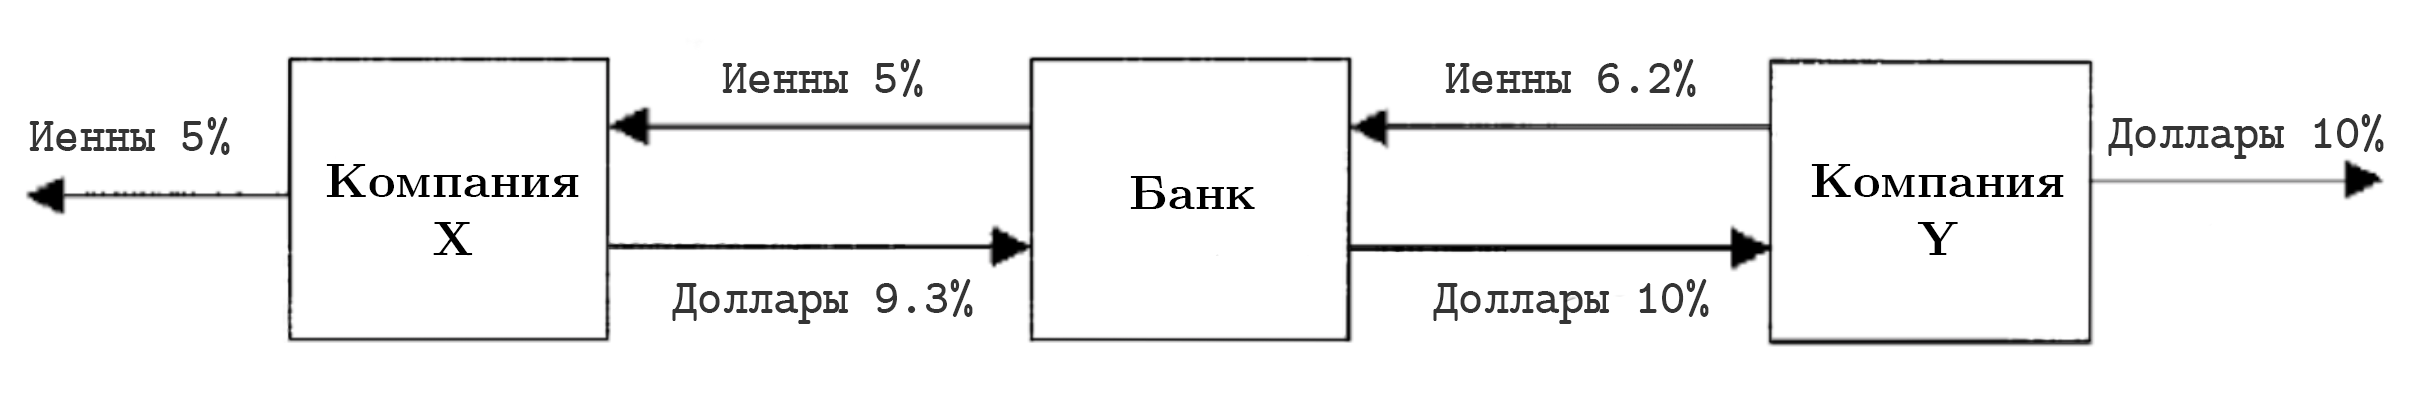
\includegraphics[width=16.7cm]{фото_курсач.png}
		\end{center}
\end{enumerate}

\newpage
\section*{4. Список литературы}
\smallskip
\begin{enumerate}
\item[{[1]}] С. В. Жуленёв, Финансовая математика. Введение в классическую теорию. Часть 2. Изд-во механико-математического факультета МГУ, 2012.
\item[{[2]}] John C. Hull, Options, Futures and Other Derivatives (6th Edition), Publishing house “Williams”, 2008.
\end{enumerate}

\end{document}